\mysection{Statistiques sur le nombre d'arguments d'une fonction}
\label{args_stat}

J'ai toujours été intéressé par le nombre moyen d'arguments d'une fonction.

\myindex{UNIX!grep}
J'ai donc analysé un bon nombre de DLLs 32 bits de Windows7\\
(crypt32.dll, mfc71.dll, msvcr100.dll, shell32.dll, 
user32.dll, d3d11.dll, mshtml.dll, msxml6.dll, sqlncli11.dll, wininet.dll, mfc120.dll, msvbvm60.dll, 
ole32.dll, themeui.dll, wmp.dll) 
(parce qu'elles utilisent la convention d'appel \emph{stdcall} et qu'il est donc facile de retrouver 
les instructions \INS{RETN X} en utilisant la commande \emph{grep} sur leur code une fois celui-ci 
désassemblé).

\begin{itemize}
\item no arguments: $\approx 29\%$
\item 1 argument: $\approx 23\%$
\item 2 arguments: $\approx 20\%$
\item 3 arguments: $\approx 11\%$
\item 4 arguments: $\approx 7\%$
\item 5 arguments: $\approx 3\%$
\item 6 arguments: $\approx 2\%$
\item 7 arguments: $\approx 1\%$
\end{itemize}

\begin{figure}[H]
\centering
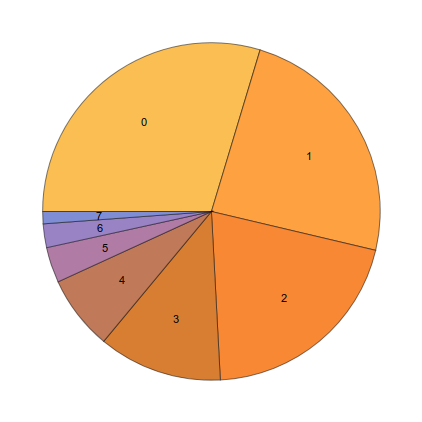
\includegraphics[width=0.5\textwidth]{other/args_stat.png}
\caption{Statistiques du nombre d'arguments moyen d'une fonction}
\end{figure}

Ces nombres dépendent beaucoup du style de programmation et peuvent s'avérer très différents pour 
d'autres logiciels.

